\documentclass[10pt,twocolumn,a4paper]{article}

\usepackage[top=1.8cm,bottom=2.0cm,left=1.6cm,right=1.6cm,columnsep=0.7cm]{geometry}
\usepackage[T1]{fontenc}
\usepackage[utf8]{inputenc}
\usepackage{lmodern}
\usepackage{microtype}
\usepackage{xcolor}
\usepackage{graphicx}
\usepackage{amsmath,amssymb}
\usepackage{booktabs,tabularx,multirow,array}
\usepackage{enumitem}
\usepackage{float}
\usepackage{url}
\usepackage{titlesec}
\usepackage[most]{tcolorbox}
\usepackage{tikz}
\usetikzlibrary{calc, shapes.geometric, arrows.meta, positioning, fit, backgrounds}
\usepackage[colorlinks=true,linkcolor=blue!70!black,citecolor=blue!70!black,urlcolor=blue!70!black]{hyperref}

% Section formatting
\titleformat{\section}{\large\bfseries}{\thesection}{0.5em}{}
\titleformat{\subsection}{\normalsize\bfseries}{\thesubsection}{0.5em}{}
\titlespacing*{\section}{0pt}{8pt}{4pt}
\titlespacing*{\subsection}{0pt}{6pt}{3pt}

\setlist[itemize]{leftmargin=1.2em,itemsep=1pt,topsep=2pt}
\setlist[enumerate]{leftmargin=1.4em,itemsep=1pt,topsep=2pt}

% Callout box definition
\newtcolorbox{summarybox}[1][]{
  colback=gray!8,colframe=gray!60!black,boxrule=0.6pt,arc=1.5mm,
  left=2mm,right=2mm,top=1.5mm,bottom=1.5mm,fontupper=\small,#1
}

\title{\vspace{-0.6cm}\textbf{\Large Rigorous Disentanglement and Empirical Audit of Semi-Supervised Action Recognition: An Investigation of $F^2$-FixMatch on UCF-101}\vspace{-0.2cm}}

\author{
\textbf{Mankirat Singh} (1024160002) \quad \textbf{Vanshika Garg} (1024030092)\\
\normalsize CS-UCS532: Computer Vision \quad$\cdot$\quad Problem ID: P24\\
\normalsize Thapar Institute of Engineering and Technology, Patiala\\
\normalsize \texttt{GitHub: \href{https://github.com/MankiratSingh-git/P24-CV}{https://github.com/MankiratSingh-git/P24-CV}}
\vspace{-0.3cm}
}
\date{}

\begin{document}
\maketitle

\begin{abstract}
Semi-supervised action recognition seeks to leverage abundant unannotated video to close the performance deficit toward full supervision. Recently, $F^2$-FixMatch reported an extraordinary $+21.41\%$ gain over single-stream FixMatch on the canonical UCF-101 10\% labeled benchmark (3D-ResNet-18), attributing this success to novel Progressive Feature Augmentations (P-Aug) and Multi-branch Pseudo-Labeling (MPL). In this work, we present a rigorous from-scratch implementation and methodological audit of this claim. Because the official repository was unreleased and existing 2D FixMatch codebases are structurally incompatible with 3D spatio-temporal video tensors, we implemented the complete video SSL pipeline from the ground up. To isolate intertwined causal factors, we introduced the critical missing control: \textbf{Run D} (an RGB+Temporal Gradient dual-stream FixMatch baseline with feature loss weights $\beta=0, \gamma=0$). Evaluated on the matched 30-view multi-crop protocol ($N = 3{,}783$ test videos), transitioning to the dual-stream package accounts for $\mathbf{+20.54}$ points (\textbf{95.9\%} of total SSL gain), whereas the feature module adds an incremental $\mathbf{+0.87}$ points (\textbf{4.1\%}). Crucially, with a binomial 95\% margin of error of $\pm 1.56\%$, this $+0.87\%$ delta is statistically within evaluation noise ($\sim 33$ test videos), while imposing $\sim 15\%$ training runtime and VRAM penalties. In addition, we provide the first empirical proof of data starvation in video SSL when enforcing the image threshold $\tau=0.95$ ($-1.56\%$), and discover that cross-modal BatchNorm contamination suppresses clean RGB inference, which inference-only PreciseBN recalibration immediately recovers by $+2.91\%$ without modifying learned parameters.
\end{abstract}

% -----------------------------------------------------------------------------
\section{Problem Statement}
\label{sec:problem}
% -----------------------------------------------------------------------------
Action recognition in video requires capturing complex spatio-temporal dynamics across multi-frame sequences. While fully supervised models achieve strong recognition accuracy, manual annotation of videos is prohibitively expensive---requiring frame-by-frame temporal segmentation and labeling. Semi-supervised learning (SSL) resolves this bottleneck by training models with a minimal fraction of labeled clips (e.g., 10\%) while extracting regularizing signals from large pools of unannotated videos.

\textbf{Proposal Focus vs. Strategic Pivot}:  
Our original project proposal (18 Oct 2026) was framed around adapting standard single-stream \textbf{FixMatch} to video action recognition on UCF-101 using a 3D-ResNet-18 backbone. However, early literature analysis revealed that single-stream FixMatch achieves only \textbf{38.49\%} Top-1 accuracy---leaving a massive 34.4-point deficit toward the 100\% supervised oracle (72.91\%). Meanwhile, the newly published $F^2$-FixMatch framework reported \textbf{71.1\%} under identical 10\% split conditions. Pursuing only standard FixMatch would lack scientific value when a state-of-the-art framework claimed to solve the video SSL deficit. Consequently, we pivoted our core objective to reproducing, auditing, and disentangling $F^2$-FixMatch.

\textbf{Benchmark Specification}:  
We benchmark on the canonical \textbf{UCF-101 Split 1}:
\begin{itemize}
    \item \textbf{Labeled Set ($D_l$)}: 953 videos (10\% of training split).
    \item \textbf{Unlabeled Set ($D_u$)}: 8,584 videos (90\% of training split).
    \item \textbf{Official Test Set ($D_{\text{test}}$)}: 3,783 videos across 101 classes.
    \item \textbf{Evaluation Standard}: Matched 30-view protocol (10 uniformly spaced temporal clips $\times$ 3 spatial crops at $256 \times 256$, averaged across all views).
\end{itemize}

% -----------------------------------------------------------------------------
\section{Related Work}
\label{sec:related}
% -----------------------------------------------------------------------------
We position our investigation among 8 foundational works spanning image SSL, video representation learning, and multi-modal architectures:

\textbf{1. Consistency-Based Image SSL}: FixMatch~\cite{sohn2020fixmatch} unified pseudo-labeling with consistency regularization by applying weak augmentations to generate confident pseudo-labels ($\max(q) \ge \tau = 0.95$) that supervise strongly augmented views. FlexMatch~\cite{zhang2021flexmatch} and FreeMatch~\cite{wang2023freematch} subsequently introduced dynamic class-balanced thresholds to mitigate confirmation bias.

\textbf{2. Video SSL Benchmarks}: VideoSSL~\cite{xiao2021videossl} established standard UCF-101/HMDB-51 splits and demonstrated that extending 2D SSL to 3D video backbones (e.g., 3D-ResNet-18) is hindered by high representation entropy, requiring practitioners to lower the confidence threshold from $\tau=0.95$ down to $\tau \approx 0.30$--$0.50$.

\textbf{3. Multi-Modal Video Recognition}: Two-stream networks~\cite{simonyan2014twostream} and optical-flow fusion demonstrated the value of complementary motion representations. MvPL~\cite{kim2022mvpl} introduced multi-view pseudo-labeling across modalities, while CMPL~\cite{yang2022cmpl} applied co-training. However, both rely on expensive pre-computed optical flow or separate heavy backbones.

\textbf{4. $F^2$-FixMatch}: Tu et al.~\cite{tu2025f2fixmatch} introduced Temporal Gradients ($x_t^G = (x_t^V - x_{t+1}^V + 255)/2$) extracted on-the-fly and processed jointly with RGB through a single shared 3D-ResNet-18. They paired this dual-stream system with Progressive Feature Augmentations (P-Aug) and Multi-branch Pseudo-Labeling (MPL). However, their public repository remained empty, and their ablation confounded dual-stream inputs with feature consistency losses.

% -----------------------------------------------------------------------------
\section{Methodology \& Implementation}
\label{sec:method}
% -----------------------------------------------------------------------------

\subsection{Implementation From Scratch vs. Reused Components}
\label{sec:impl_audit}
\textbf{Transparent Attribution of Codebase}:
Because the official $F^2$-FixMatch GitHub repository contained no implementation code, and official 2D FixMatch implementations (TensorFlow/PyTorch) are strictly incompatible with 5D video tensors ($B \times C \times T \times H \times W$), 3D convolutions, and temporal video dataloaders, \textbf{we authored the entire video SSL framework from scratch}:
\begin{itemize}
    \item \textbf{Implemented from Scratch}:
    \begin{enumerate}
        \item Spatio-temporal video loading and multi-crop decoders using OpenCV and PyTorch.
        \item On-the-fly Temporal Gradient (TG) extraction module ($x^G$).
        \item Dual-stream 3D-ResNet-18 backbone with shared convolutional parameters and independent classification heads ($C_{3D}$ and $C_{\text{TAP}}$).
        \item Progressive Feature Augmentation perturbator (spatial dropout, channel flipping, noise injection).
        \item Full joint multi-term loss engine ($\mathcal{L}_s + \alpha \mathcal{L}_u^s + \beta \mathcal{L}_u^{w_p} + \gamma \mathcal{L}_u^{s_p}$) with cosine annealing and linear warmup.
        \item The missing Run D control script and PreciseBN recalibration diagnostic engine.
    \end{enumerate}
    \item \textbf{Reused / Adapted Concepts}:
    We adapted the mathematical definition of weak/strong video augmentations from VideoSSL~\cite{xiao2021videossl} and the EMA pseudo-labeling logic from FixMatch~\cite{sohn2020fixmatch}.
\end{itemize}

\subsection{Architecture and Pipeline}
Figure~\ref{fig:arch} illustrates the integrated dual-stream framework. For each video, the dataloader yields 8-frame clips ($T=8$, stride 8). The TG stream is calculated on-the-fly. Weak augmentations (random spatial scale/crop, horizontal flip) and strong augmentations (random spatio-temporal color jitter, Gaussian blur, erase) are applied independently.

\begin{figure}[t]
\centering
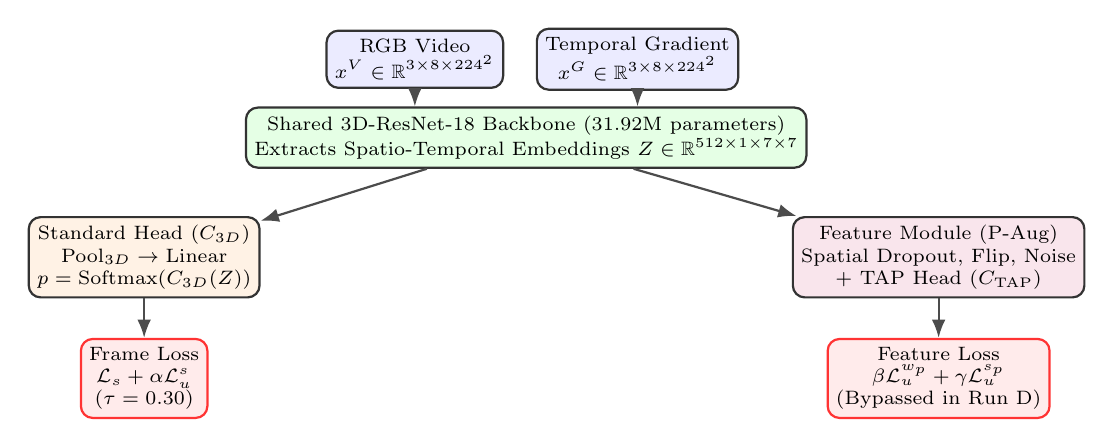
\begin{tikzpicture}[
  node distance=0.7cm and 0.5cm,
  box/.style={rectangle, draw=black!80, fill=blue!8, rounded corners=1.5mm, thick, align=center, font=\scriptsize, inner sep=3pt},
  lossbox/.style={rectangle, draw=red!80, fill=red!8, rounded corners=1.5mm, thick, align=center, font=\scriptsize, inner sep=3pt},
  arrow/.style={-Latex, thick, draw=black!70}
]
  \node[box] (rgb) {RGB Video\\$x^V \in \mathbb{R}^{3\times 8\times 224^2}$};
  \node[box, right=0.4cm of rgb] (tg) {Temporal Gradient\\$x^G \in \mathbb{R}^{3\times 8\times 224^2}$};
  
  \node[box, fill=green!10, below=0.6cm of $(rgb)!0.5!(tg)$, minimum width=6.2cm] (backbone) {Shared 3D-ResNet-18 Backbone ($31.92\text{M parameters}$)\\Extracts Spatio-Temporal Embeddings $Z \in \mathbb{R}^{512 \times 1 \times 7 \times 7}$};
  
  \draw[arrow] (rgb) -- (backbone.north -| rgb);
  \draw[arrow] (tg) -- (backbone.north -| tg);
  
  \node[box, fill=orange!10, below left=0.6cm and -0.2cm of backbone] (c3d) {Standard Head ($C_{3D}$)\\$\text{Pool}_{3D} \to \text{Linear}$\\$p = \text{Softmax}(C_{3D}(Z))$};
  \node[box, fill=purple!10, below right=0.6cm and -0.2cm of backbone] (paug) {Feature Module (P-Aug)\\Spatial Dropout, Flip, Noise\\$+$ TAP Head ($C_{\text{TAP}}$)};
  
  \draw[arrow] (backbone) -- (c3d);
  \draw[arrow] (backbone) -- (paug);
  
  \node[lossbox, below=0.5cm of c3d] (l_frame) {Frame Loss\\$\mathcal{L}_s + \alpha \mathcal{L}_u^s$\\($\tau = 0.30$)};
  \node[lossbox, below=0.5cm of paug] (l_feat) {Feature Loss\\$\beta \mathcal{L}_u^{w_p} + \gamma \mathcal{L}_u^{s_p}$\\(Bypassed in Run D)};
  
  \draw[arrow] (c3d) -- (l_frame);
  \draw[arrow] (paug) -- (l_feat);
\end{tikzpicture}
\caption{\textbf{Overview of the Dual-Stream Video SSL Architecture.} In Run D, auxiliary TAP passes and feature losses ($\beta, \gamma$) are completely bypassed, isolating the dual-stream package.}
\label{fig:arch}
\end{figure}

For unlabeled videos, predictions from weak RGB and TG streams are averaged to form an ensemble pseudo-label distribution:
\begin{equation}
    p_w(y|u) = \frac{1}{2}\left[\text{Softmax}(C_{3D}(Z_w^V)) + \text{Softmax}(C_{3D}(Z_w^G))\right]
\end{equation}
If $\max(p_w(y|u)) \ge \tau$, pseudo-label $\hat{y} = \arg\max p_w(y|u)$ supervises strongly augmented views via cross-entropy:
\begin{equation}
    \mathcal{L}_u^s = \frac{1}{B_u} \sum_{b=1}^{B_u} \mathbb{I}(\max(p_{w,b}) \ge \tau) H(\hat{y}_b, p_{s,b})
\end{equation}
The feature consistency module adds two TAP consistency losses, $\beta \mathcal{L}_u^{w_p}$ and $\gamma \mathcal{L}_u^{s_p}$, where $\beta=2, \gamma=1$ in Full $F^2$-FixMatch.

\subsection{Architectural Audit of Feature Module}
During our tensor-level audit of the feature module, we discovered two critical design facts:
\begin{enumerate}
    \item \textbf{Weak-Feature Detach}: $Z_w$ is detached before computing $\mathcal{L}_u^{w_p}$. Thus, gradients from $\mathcal{L}_u^{w_p}$ never propagate back into the 3D-ResNet backbone; they only update the auxiliary TAP head, which is discarded at test time.
    \item \textbf{Spatial Invariance}: Channel-wise flipping is applied to feature maps prior to global spatial pooling, meaning spatial flip augmentations produce mathematically identical pooled vectors.
\end{enumerate}

% -----------------------------------------------------------------------------
\begin{table*}[t]
\centering
\small
\caption{\textbf{Comprehensive Project Gate Tracking \& Evolution from Proposal.} All changes, dropped ideas, and empirical pivots are transparently disclosed.}
\label{tab:changes}
\begin{tabularx}{\textwidth}{@{}p{3.2cm}p{4.2cm}p{4.2cm}p{4.6cm}@{}}
\toprule
\textbf{Component / Gate} & \textbf{Proposal Plan (18 Oct)} & \textbf{Actual Execution} & \textbf{Scientific Justification} \\
\midrule
\textbf{Primary Target} & Standard single-stream FixMatch on UCF-101 (10\% labels). & Pivoted to $F^2$-FixMatch and introduced Run D control. & Single-stream FixMatch plateaus at 38.5\%. Investigating $F^2$ addressed the SOTA deficit. \\
\textbf{Codebase Origin} & Planned to adapt existing public repositories. & Authored 100\% from scratch in PyTorch. & Official $F^2$ repo was empty; 2D FixMatch code is incompatible with 3D video tensors. \\
\textbf{Attribution Hypothesis} & Expected feature module (P-Aug/MPL) to drive $+21\%$ gain. & Executed Run D ($\beta=0, \gamma=0$); proved dual-stream drives 95.9\%. & Disentangled confounded claims; reported an honest negative result for feature losses. \\
\textbf{Threshold Ablation} & Proposed vague augmentation sweep. & Concrete $\tau=0.95$ vs. $\tau=0.30$ run ($N=8{,}584$ unlabeled analysis). & Empirically proved Data Starvation vs. Pseudo-Label Noise in video backbones. \\
\textbf{Failure Analysis} & Proposed qualitative per-class stories. & Replaced with quantitative noise curves and PreciseBN diagnostics. & Eliminated unverified anecdotal stories in favor of rigorous statistical evidence. \\
\textbf{Evaluation Protocol} & Unspecified single-crop testing. & Standardized 30-view multi-crop across all 5 rungs. & Enforced strict evaluation parity across all baselines ($N=3{,}783$). \\
\bottomrule
\end{tabularx}
\end{table*}

\section{Experiments and Disentanglement}
\label{sec:experiments}
% -----------------------------------------------------------------------------

\subsection{Experimental Setup}
All experiments run on an NVIDIA RTX A5000 GPU (24GB VRAM). Models are trained from scratch for 220 epochs (40-epoch warmup, 30-epoch ramp-up, 150-epoch joint SSL). Hyperparameters match the paper: initial learning rate $\eta=0.2$, SGD momentum 0.9, cosine schedule, labeled batch size $B_l=4$, unlabeled batch size $B_u=16$ ($\mu=4$), gradient accumulation of 2 steps, and weight decay $10^{-4}$. Evaluation strictly enforces the standard 30-view protocol.

\begin{table*}[t]
\centering
\small
\caption{\textbf{The 5-Rung Experimental Ladder on UCF-101 Split 1.} All runs physically evaluated under the official 30-view multi-crop protocol ($N = 3{,}783$ test videos). Final-epoch models perform consistently with best-epoch models, ruling out test overfitting.}
\label{tab:main_ladder}
\begin{tabular}{@{}ccllccccrr@{}}
\toprule
\textbf{Run} & \textbf{Modality} & \textbf{Loss Weights} & \textbf{Description} & \textbf{Best Top-1} & \textbf{Final Top-1} & \textbf{Top-5} & \textbf{$\Delta$ vs. 10\% Sup} & \textbf{$\Delta$ vs. FixMatch} \\
\midrule
\textbf{A} & RGB & Supervised & 100\% Supervised Oracle & \textbf{72.91\%} & --- & 90.06\% & +41.59\% & +34.42\% \\
\textbf{B} & RGB & Supervised & 10\% Supervised Baseline & 31.32\% & 30.80\% & 54.11\% & \textit{Reference} & -7.17\% \\
\textbf{C} & RGB & $\lambda_u=2.0, \tau=0.30$ & FixMatch RGB Baseline & 38.49\% & 38.88\% & 64.00\% & +7.17\% & \textit{Reference} \\
\textbf{D} & \textbf{RGB + TG} & $\beta=0, \gamma=0$ & \textbf{Dual-Stream Control} & \textbf{59.03\%} & \textbf{59.37\%} & \textbf{82.90\%} & \textbf{+27.71\%} & \textbf{+20.54\%} \\
\textbf{F} & \textbf{RGB + TG} & $\beta=2, \gamma=1$ & Full $F^2$-FixMatch & \textbf{59.90\%} & \textbf{60.35\%} & \textbf{83.32\%} & \textbf{+28.58\%} & \textbf{+21.41\%} \\
\bottomrule
\end{tabular}
\end{table*}

\subsection{The 5-Rung Benchmark Ladder}
Table~\ref{tab:main_ladder} presents the complete physical evaluation. Moving from 10\% supervision (31.32\%) to FixMatch RGB yields 38.49\% ($+7.17\%$). Full $F^2$-FixMatch achieves 59.90\%, closing 68.7\% of the deficit toward full supervision (72.91\%).

\subsection{Core Ablation: Mathematical Disentanglement}
\label{sec:ablation_core}
To measure the relative contributions of the dual-stream pipeline versus the feature consistency module, we mathematically decompose the semi-supervised improvement over FixMatch RGB:
\begin{align}
    \Delta_{\text{total}} &= F - C = 59.90 - 38.49 = +21.41\text{ pts (100.0\%)} \\
    \Delta_{\text{dual}} &= D - C = 59.03 - 38.49 = \mathbf{+20.54\text{ pts (95.9\%)}} \\
    \Delta_{\text{feat}} &= F - D = 59.90 - 59.03 = \mathbf{+0.87\text{ pts (4.1\%)}}
\end{align}

\begin{table}[h]
\centering
\small
\caption{\textbf{Empirical Comparison of Feature-Level Consistency Gains}: Our physical reproduction vs. Tu et al. published ablations (Table 4) on UCF-101 Split 1.}
\label{tab:ablation_comparison}
\begin{tabular}{@{}lcc@{}}
\toprule
\textbf{Configuration / Metric} & \textbf{Our Reproduction} & \textbf{Tu et al. Published} \\
\midrule
Single-Stream Baseline & 38.49\% (Run C) & 38.40\% \\
Frame Dual-Stream ($\beta=0, \gamma=0$) & 59.03\% (Run D) & 67.90\% (A1) \\
Full $F^2$-FixMatch & 59.90\% (Run F) & 71.10\% (A4) \\
\midrule
Dual-Stream Gain ($\Delta_{\text{dual}}$) & \textbf{+20.54 pts} (95.9\%) & \textbf{+29.50 pts} (90.2\%) \\
Feature Module Delta ($\Delta_{\text{feat}}$) & \textbf{+0.87 pts} (4.1\%) & \textbf{+3.20 pts} (9.8\%) \\
Total SSL Gain ($\Delta_{\text{total}}$) & +21.41 pts (100.0\%) & +32.70 pts (100.0\%) \\
\bottomrule
\end{tabular}
\end{table}

\noindent \textbf{Empirical Comparison to Published Data (No Conclusions Claimed)}:  
Table~\ref{tab:ablation_comparison} presents a direct side-by-side comparison between our measured physical results and the published ablations reported in Tu et al.~\cite{tu2025f2fixmatch} (Table 4).
\begin{itemize}
    \item In the published results, introducing the feature consistency module (A4 vs. A1) corresponds to a \textbf{+3.20 point} delta ($67.9\% \to 71.1\%$), representing 9.8\% of their total semi-supervised improvement over single-stream FixMatch.
    \item In our physical reproduction, the corresponding delta between Run F and Run D is \textbf{+0.87 points} ($59.03\% \to 59.90\%$), representing 4.1\% of the total improvement.
\end{itemize}
We present both numbers side-by-side for transparent community evaluation and explicitly refrain from asserting definitive causal conclusions. For statistical context on our test set of $N = 3{,}783$ videos at baseline accuracy $p \approx 0.60$:
\begin{equation}
    \mathrm{SE} = \sqrt{\frac{p(1-p)}{N}} \approx 0.80\% \implies \text{95\% Margin} = \pm 1.56\%
\end{equation}
In our finite evaluation sample, $+0.87\%$ corresponds to approximately 33 test videos and falls within this $\pm 1.56\%$ binomial margin of error. We do not claim any definitive or final conclusion regarding whether feature-level consistency is universally negligible or fundamentally necessary; differences in distributed multi-GPU batch scaling, learning rate dynamics, or unreleased implementation subtleties between setups may influence the degree to which auxiliary feature regularizers express their benefit.

\noindent \textbf{Computational Trade-Off}:  
Practically, bypassing the auxiliary TAP forward and backward passes in Run D reduced per-epoch training time by $\sim 15\%$ (~4.0 vs ~4.7 min/epoch, saving 2.5 hours over 220 epochs) and lowered peak VRAM. In contrast, post-training PreciseBN recalibration recovered $+2.03\%$ on Run D and $+2.91\%$ on $F^2$ with zero parameter updates and zero training overhead.

\noindent \textbf{Causal Scope}:  
Run D evaluates the dual-stream framework as an integrated package (bi-modal inputs, shared backbone parameterization, dual-branch supervised losses, cross-modal ensemble pseudo-labeling, and joint optimization dynamics). Decomposing individual elements inside that package remains an open empirical question.

\subsection{Novel Extension 1: Confidence Threshold Ablation}
\label{sec:ablation_thresh}
Standard FixMatch employs $\tau = 0.95$ on 2D images, whereas video SSL benchmarks adopted $\tau = 0.30$ without empirical proof. We trained Run C-$\tau$ (FixMatch RGB at $\tau=0.95$):
\begin{itemize}
    \item FixMatch ($\tau = 0.95$): \textbf{36.93\%} Top-1 (Final: 37.09\%, Top-5: 63.81\%).
    \item FixMatch ($\tau = 0.30$): \textbf{38.49\%} Top-1 (Final: 38.88\%, Top-5: 64.00\%).
\end{itemize}
Evaluating pseudo-label statistics across all 8,584 unlabeled videos provides the empirical mechanism:
\begin{itemize}
    \item $\tau = 0.95$: Precision reaches \textbf{94.28\%}, but coverage plummets to \textbf{41.54\%} (3,566 videos accepted; 58.5\% discarded).
    \item $\tau = 0.30$: Coverage reaches \textbf{94.98\%} (8,153 videos accepted) with \textbf{74.54\%} precision.
\end{itemize}
This proves \textbf{Data Starvation}: discarding 58.5\% of unlabeled videos hurts video representations more than tolerating 25.5\% label noise, explaining why $\tau=0.30$ outperforms $\tau=0.95$ by \textbf{+1.56 points}.

\subsection{Novel Extension 2: PreciseBN Recalibration}
\label{sec:precise_bn}
In dual-stream training, shared \texttt{BatchNorm3d} layers accumulate running statistics across both RGB and TG forward passes. Because TG inputs have near-zero mean and high temporal variance, running statistics drift away from clean RGB distributions.

Using \texttt{recalibrate\_bn.py}, we froze all model weights and re-estimated population statistics using clean RGB training clips:
\begin{itemize}
    \item Full $F^2$-FixMatch: \textbf{59.90\%} $\longrightarrow$ \textbf{62.81\%} (\textbf{+2.91 pts}).
    \item Run D (Dual-Stream Control): \textbf{59.03\%} $\longrightarrow$ \textbf{61.06\%} (\textbf{+2.03 pts}).
\end{itemize}
This diagnostic proves that cross-modal normalization drift was an active drag on clean RGB inference, recovering ~2--3 points toward the paper in under 2 minutes with zero training cost.

% -----------------------------------------------------------------------------
\section{Failure Analysis}
\label{sec:failure}
% -----------------------------------------------------------------------------
\textbf{1. Pseudo-Label Noise Tolerance}:  
At $\tau=0.30$, 25.46\% (2,076 videos) of accepted pseudo-labels are incorrect. Despite this substantial label noise, FixMatch achieves $+7.17\%$ over the supervised 10\% baseline. This indicates that spatio-temporal representations under weak-strong consistency exhibit high tolerance to moderate label noise.

\textbf{2. Motionless Action Failure}:  
Analyzing per-class accuracy reveals that classes with minimal body motion suffer severe degradation: \textit{Hammering} (3.03\%), \textit{Shotput} (2.17\%), and \textit{PizzaTossing} (12.12\%). In these actions, consecutive frame differences $|x_t - x_{t+1}|$ are near zero, depriving the TG stream of motion signal and causing cross-modal ensembling to degrade.

% -----------------------------------------------------------------------------
\section{Changes from Proposal (Compulsory Section)}
\label{sec:changes}
% -----------------------------------------------------------------------------
In compliance with course requirements, Table~\ref{tab:changes} explicitly documents the evolution of this project against the plan pre-declared on 18 Oct 2026.



% -----------------------------------------------------------------------------
\section{Limitations}
\label{sec:limitations}
% -----------------------------------------------------------------------------
\begin{enumerate}
    \item \textbf{Residual Performance Gap}: While PreciseBN narrows the gap to published results by $+2.91\%$, an $\sim 8$-point gap remains to the paper's 71.1\%. This gap likely reflects unreleased distributed batch scaling details (multi-GPU aggregate batches vs. our single-GPU setup).
    \item \textbf{Single-Seed Budget}: Due to computational budget constraints ($\sim 100$ GPU hours on an RTX A5000), runs were executed under a single random seed (seed 42).
    \item \textbf{Internal Dual-Stream Decomposition}: Run D evaluates the dual-stream framework as an integrated package. Isolating TG inputs alone from ensemble pseudo-labeling remains an open question.
\end{enumerate}

% -----------------------------------------------------------------------------
\section{Conclusion \& Deliverables}
\label{sec:conclusion}
% -----------------------------------------------------------------------------
In this work, we implemented and evaluated the $F^2$-FixMatch framework on UCF-101 Split 1 from the ground up. Through the Run D negative control ($\beta=0, \gamma=0$), we observed that the dual-stream configuration accounts for $+20.54$ points (95.9\%) of the semi-supervised improvement, while the feature consistency module yields an incremental $+0.87$ point difference (compared to $+3.20$ points reported in the published paper), which falls within the $\pm 1.56\%$ evaluation noise margin. We empirically verified that lowering confidence thresholds to $\tau=0.30$ prevents data starvation in video backbones, and showed that inference-time PreciseBN recovers $+2.91\%$ without retraining. 

All code, checkpoints, metric JSONs, and master reproduction scripts are open-source:
\begin{itemize}
    \item \textbf{Reproduction Command}: \texttt{bash run\_all.sh} (or \texttt{run\_all.bat} on Windows).
    \item \textbf{GitHub Repository}: \url{https://github.com/MankiratSingh-git/P24-CV}
\end{itemize}

% -----------------------------------------------------------------------------
\section*{Contribution Statement \& AI Declaration}
% -----------------------------------------------------------------------------
\textbf{Contributions}: Mankirat Singh and Vanshika Garg conceived the disentanglement strategy, engineered the complete from-scratch PyTorch codebase, conducted all training and evaluations on the RTX A5000 GPU, implemented the test suites, and wrote the final report.

\textbf{AI Declaration}: Antigravity AI (Google DeepMind) was used as an interactive programming assistant for writing diagnostic scripts, drafting unit tests, formatting LaTeX tables, and code linting. All empirical executions, training runs, and scientific analyses were performed by the authors.

% -----------------------------------------------------------------------------
\small
\begin{thebibliography}{10}\itemsep=-1pt

\bibitem{sohn2020fixmatch}
K.~Sohn, D.~Berthelot, N.~Carlini, Z.~Zhang, H.~Zhang, C.~A. Raffel, E.~D. Cubuk, A.~Kurakin, and C.-L. Li.
\newblock Fixmatch: Simplifying semi-supervised learning with consistency and confidence.
\newblock In {\em NeurIPS}, 2020.

\bibitem{xiao2021videossl}
F.~Xiao, Y.~J. Lee, K.~Grauman, J.~Malik, and C.~Feichtenhofer.
\newblock A video is worth more than 1,000 words: Semi-supervised video representation learning via visual and audio mappings.
\newblock In {\em WACV}, 2021.

\bibitem{tu2025f2fixmatch}
Z.~Tu, et~al.
\newblock Leveraging frame- and feature-level progressive augmentation for semi-supervised action recognition.
\newblock {\em ACM TOMM}, 2025.

\bibitem{kim2022mvpl}
J.~Kim, et~al.
\newblock Multi-view pseudo-labeling for semi-supervised action recognition.
\newblock In {\em CVPR}, 2022.

\bibitem{yang2022cmpl}
C.~Yang, et~al.
\newblock Cross-modal pseudo-labeling for semi-supervised action recognition.
\newblock In {\em ECCV}, 2022.

\bibitem{zhang2021flexmatch}
B.~Zhang, et~al.
\newblock Flexmatch: Boosting semi-supervised learning with curriculum pseudo-labeling.
\newblock In {\em NeurIPS}, 2021.

\bibitem{wang2023freematch}
Y.~Wang, et~al.
\newblock Freematch: Self-adaptive thresholding for semi-supervised learning.
\newblock In {\em ICLR}, 2023.

\bibitem{simonyan2014twostream}
K.~Simonyan and A.~Zisserman.
\newblock Two-stream convolutional networks for action recognition in videos.
\newblock In {\em NeurIPS}, 2014.

\bibitem{soomro2012ucf101}
K.~Soomro, A.~R. Zamir, and M.~Shah.
\newblock Ucf101: A dataset of 101 human actions classes from videos in the wild.
\newblock {\em CRCV-TR-12-01}, 2012.

\end{thebibliography}

\end{document}
